\documentclass[10pt,twocolumn]{article} % removed a4 option (is default)

\usepackage[margin=1.5cm]{geometry}
\usepackage{nameref}
\usepackage{hyperref}
\usepackage{titlesec}
\usepackage{graphicx}
\usepackage{enumitem}
\usepackage{xurl}
\usepackage{todonotes}

% Set heading spacings, please don't change this
\titlespacing\section{0pt}{8pt plus 4pt minus 2pt}{0pt plus 2pt minus 2pt}
\titlespacing\subsection{0pt}{8pt plus 4pt minus 2pt}{0pt plus 2pt minus 2pt}
\titlespacing\subsubsection{0pt}{8pt plus 4pt minus 2pt}{0pt plus 2pt minus 2pt}

\author{
  Belinda Kneubühler (2504756K), Ben Hanmer (2505218H),\\
  Daniels Vasiljevs (2500414V), Shaun Loughery (2193422L),\\
  Zsuzsanna Szugyi (2418750S)}

\title{Puzzle Map}
\date{} % Leave empty

\begin{document}

\maketitle


% ------------------------------------
\section*{Introduction}

This is the template for the MHCI coursework report.


% ------------------------------------
\section*{Purpose}

The main purpose of the product is to create an interactive, gamified mobile application for the discovery of the University campus that helps students and staff learn more about the University in an individual or group setting. It is developed to promote discovering the whole of the university in choosable paths and speeds,  and to encourage social activities as opposed to lone solutions. It is to be available for any current or prospective student and staff - all registered at the university with a GUID - , but the main target demographic are new students.\\
The system is based on a remote database which stores the details of the locations and users, and this data is served to the user in the form of a mobile device application, as this provides the best user experience (UX).

% ------------------------------------
\section*{System Description}

\subsection*{Functionality}
Users can access the app by creating an account using their university email (specifically, GUID). The app allows for not only the creation of the account, but the maintenance (forgotten password, change details, etc.), and deletion of it. Users have to fill out a personality quiz, the answers of which will later on bias the likelyhood of what location a user will most likely get offered to head to next. The app will make it possible to read an interactive checkpoint, e.g. AR tag, which would prompt a riddle to the user that they need to solve. In the possibility of the puzzle being too hard to decipher, there are 3 hints available for each, which make the puzzle gradually easier to solve. The app will also allow for users to increase their in-game experience by correctly solving riddles, and use the experience to level up and gain rewards by doing well in the app. The system also allows for and promotes social interactions between users, to work together to a shared goal of successfully solving a riddle.\\
Aspects that entertain and engage the user include the riddles/puzzles, AR and the checkpoints, achievements and online character development, friend connections and gifting, freebies and rewards to gain, and the learning of insider information about the campus.

\subsection*{User characteristics and needs}
The goals of the users would be to visit as many locations on campus as possible, and do it in the most efficient way gaining the most bonus from solving riddles correctly. This would give them increased chances to gain freebies, level up and develop their level of experience, which would keep them captivated, entertained and interested. New students and faculty would use the app to get more information about the campus, while existing university members would use the app to either learn about the university with a delay, or to put their existing knowledge to use to gain as many points as possible and get the rewards.\\
The main motivation, however, of any type of user is likely to be the love of mysteries, problem solving, and the possibility to pass the time in a fun way and interact with peers with a more relaxed environment than social media. In the case of any users, however, it can be assumed that they have a busy lifestyle and therefore the app is a series of short tasks without expiry dates, which can fit around any student/staff member's schedule.

\subsection*{Constraints}
The two biggest constraints to the operations of the app are the user's device capabilities, and the reliability of internet connectivity. These are both aspects the app needs to be designed for, to minimise the disruption these constraints would mean. Since users can walk freely around campus, gepgraphical and physical obstacles do not represent significant constraints.

\subsection*{Assumptions and dependencies}
The system and its operations can be affected by many external entities. This includes user device capabilities, the weather (if used when walking), developments in AR/MR technology, University redevelopment (buildings built/torn down, rooms made available/unavailable), and the user leaving the university having not completed the game yet.

\section*{Requirements}

\subsection*{Functional requirements}
The following are the main functional requirements the system has to fit:
\begin{itemize}[noitemsep]
  \item The system needs to scan the AR tag/QR code/etc.
  \item The system needs to randomly choose a building/riddle based on category
  \item The system needs to register category chosen
  \item The system needs to register personality test results
  \item The system needs to respond randomly with bias from personality test
  \item The system needs to register the riddle being solved/not solved
  \item The system needs to update user profile based on solved/not solved riddle
  \item The system needs to update user profile in relation to freebies, levels, achievements
  \item The system needs to handle account creation and logins
  \item The system needs to communicate with a database to store all data
  \item The system needs to communicate online
\end{itemize}

\subsection*{Non-functional requirements}
Non-functional requirements may not relate directly to the system's operations, but are equally important to consider for a good UX. It has been shown loading times affect the number of users retained by a service\footnote{\url{https://developers.google.com/web/fundamentals/performance/why-performance-matters}}. Therefore the following performance limits were set for the app, speedwise: the system should login in <5s, recognise tags in <5s, and complete the initialisation (show splash screen) in <20s.\\
It is also key to calculate for errors that might happen. To ensure users are never left in the dark, in case an unexpected issue were to happen, the system must show an error page with a clear message on what has happened, and what should be done by the user to mitigate it (e.g. "Uh-oh, something puzzled our app! Please leave feedback here <link>!".
\subsection*{Safety and Security}
While the design of the app focuses on most interactions happening when the user is stationary by a checkpoint, it allows for it to be used when the user is mobile (check map, friends status, etc.). To ensure the safety of the users, the app therefore does not require to be constantly watched. This is complemented by the non-linearity of the application, as the user can choose their own path, and therefore can avoid unsafe areas. The system also needs to be protected to avoid the loss of data, therefore the remote database requires regular backups - this can be supported by the user data being stored on the device locally.
\subsection*{Quality, maintainability and availability}
The quality of the product is the final aspect focused on. It was determined that not only the database and the app should be available at all times, but the checkpoints, too. These naturally vary based on building opening times, but the app has to provide satisfactory information on when checkpoints may not be available. The system also needs to correctly relay and register checkpoint location information, as well as be easily adjustable and maintainable for the adding and removal of checkpoints. 



% ------------------------------------
\section*{Concept Generation}
Lorem ipsum dolor sit amet, consectetur adipiscing elit, sed do eiusmod tempor incididunt ut labore et dolore magna aliqua. Ut enim ad minim veniam, quis nostrud exercitation ullamco laboris nisi ut aliquip ex ea commodo consequat. Duis aute irure dolor in reprehenderit in voluptate velit esse cillum dolore eu fugiat nulla pariatur. Excepteur sint occaecat cupidatat non proident, sunt in culpa qui officia deserunt mollit anim id est laborum.

% ------------------------------------
\section*{Initial Prototyping} \todo{We only did paper prototypes in this stage, I would suggest to rename this section "Paper Prototyping and remove the next subsection header.}
\subsection*{Paper Prototypes}
Once the inital design ideas were agreed upon, the ideas can then be represented as paper prototypes. Each team member is reponsible with designing their own interaction prototypes that represents the previously agreed design choices.

Each team member presented their paper prototypes to the other team members. The paper prototypes were based on an imaginary story of a user on the app. The prototypes were evaluated based on several criteria \todo{what criteria? specify, otherwise delete} that determines the usability of the app. These prototypes are all available for reference in Appendix A.

\subsection*{Prototype 1 (bens)}
The first prototype generated focusses on maintaining the map as the center of the user's view. The map will almost always be visible regardless of what the user wishes to do. The main interactive elements of the screen are located at the bottom of the screen. The only exception of this rule is that the settings button will be located at the top-left side of the screen.

The user can press the buttons at the bottom of the screen to navigate to the different sections of the screen. The user will always be within one or two screens away from the main map view. The buttons located at the bottom of the screen include: a home buton to return to the main map view; a button to view the current destination and available riddle; a button to initiate the camera module; a button to access a list of currently available offers and a button to access the profile.

\subsection*{Prototype 2 (daniels)}
Prototype two was split amongst more frames and was more focussed on keeping the screen from being cluttered. The user is greeted with a splash screen with a loading bar to show the current progress of loading the app. The user will then be guided to a signup/login screen. Once the user logs in for the first time, a quiz is displayed. This quiz will have questions and answers ranging from: strongly agree; agree; disagree and strongly disagree. Additionally, there will also be a progress indicator that shows the user how many questions are remaining. 

Once the user has finished the initial quiz, they will be given the option to select a riddle. Once the user selects a riddle, the question is displayed on the screen. The user can swipe left from this screen to access a list of available hints and unlock any other hints they require. The user can also swipe right and access the camera. This camera is used to take a picture of the AR code to complete the riddle. 

In addition to these screens, the user will also be able to access their profile. This will contain relative information about the user such as their username and profile picture. The user will always have a back button to escape back to the view containing the current riddle.

\subsection*{Prototype 3 (zsuzsi)}
Paper prototype three is more focussed on user interactivity. When the user initially starts the application, they are greeted with a splash screen with the app logo. This splash screen converts into a login screen for the user. The users are also given an option to create an account.

Once the user logs into their account, they are shown the main screen of the app. This screen has a list of options for the user to select from. If it is the user's first time using the app, a button labelled "get started" which the user will be directed to find a valid AR tag. Otherwise, if the user has already initiated a riddle, they can access their current riddle from that screen. There is a "profile" button which can show the user their profile and all the achievements they have gained. Additionally, there is a "settings" button which takes the user to a page that has all the settings that can be modified to change the game mechanics.

When the user is asked to select a location, they are shown a screen which gives them three options: Lab; Lecture or social.

Once the user has selected a riddle, the riddle is shown on screen. The user has a set number of hints and as they use these hints, the riddle changes and becomes easier to solve. The user can then choose to solve the riddle at any point by swiping up from the bottom to open the camera. 

Once the user scans the AR code, the app will inform them if they have been successful and scanned the correct location. The app will also inform them if they have levelled up and any free offers they have unlocked.

\subsection*{Prototype 4 (shaun)}
This prototype also focussed heavily on maintaining a minimilistic design. This prototype uses many different screens to display information. 

The prototype has an initial start screen with a button to continue to the login screen. This login screen has an option to remember the user. Once the user logs in, if this is their first time using the app, they are displayed with a personality quiz. Otherwise, the main screen is shown.

The main screen consists of the main map view and the logo of the app. This screen also hosts a floating action button that can be used to open the camera module. If the user opens the camera, a basic AR scanner is shown on screen. 

Once a user scans a valid AR tag, they are shown with a screen that details information about the area and informs the user about the amount of XP they have gained. The user can then press a button to continue and the app will give them four buttons that can be selected to direct where they want to go. Once the user has selected a location, the main screen will show again and the riddle for the new location will be shown on screen overlaying the map.

The profile can be accessed through the settings menu. This profile will display: the user's name; the user's profile picture; the basic information held about the user; the user's friend list and a back button to return to the main map screen.

\subsection*{Prototype 5(belinda)}

The final prototype suggested had a similar structure to the previous prototypes. A minimalistic design was implemented for the initial use of the app. The user would be greeted with two buttons; one to sign up and one to log in. When the user has signed in for the first time they will be greeted with a quiz.

After they complete this quiz, they will be greeted with the main view of the app. This consists of a main map view with several buttons at the top and bottom of the screen. The buttons at the top of the screen will give the user the option to select a lab, lecture or social based riddle. The user will not be limited to one riddle at a time to allow them to revisit riddles that they can not currently solve. The key points will be highlighted on the map as starts.

The bottom part of the screen will swipe up to reveal a navigation drawer. This drawer will contain buttons that can be used to navigate to the other parts of the application. For example, a hints button will give them tips for the current riddle. A camera button will be visible which allows the user to scan an AR code. This AR code will signify the user completing the riddle. Additionally, if the user scans an incorrect AR code, they will be given the option to claim the reward anyway or leave and come back. Another button could be visible which shows the user their currently available offers. The user will also be able to access their profile from this navigation bar. Their profile will show their name, icon and their current skill levels.

\subsection*{Testing the Prototypes}
Each of these paper prototypes were evaluated within the team. These ideas were discussed and the good and the bad interactions were noted for the refined prototype.

\subsubsection*{Good}
\begin{itemize}[noitemsep]
  \item Keep the design simple
  \item Allow the user to always be able to access the main map
  \item Keep a navigation bar accessable at the bottom of the screen with intuitive buttons
  \item Give the user access to always visit locations regardless of their current riddle state
  \item Reward the user for visiting locations regardless if they solved the riddle or note
  \item Provide a motive to the user to solve the riddles, such as extra experience points
  \item Provide the user with several riddles so that they are not stuck on one specific riddle
  \item Keep the splash screen minimal and make it automatically disappear rather than remain persistent
  \item Provide features that encourage making new friends
  \item Provide offers to the user to encourage them to keep using the application
  \item Give the user the option on what to do next after they solve the riddle
\end{itemize}

\subsubsection*{Bad}
\begin{itemize}[noitemsep]
  \item A map must be provided
  \item Do not use swiping motions close to the edges of the screens due to gestures built within the smart phone systems
  \item Do not use an excessive amount of on screen elements as this may confuse the user
  \item Do not provide only one riddle
  \item Having the settings menu as a persistent button clutters the screen and can be relocated elsewhere
  \item Do not punish the user heavily for not solving the riddle
  \item If the user accidentally answers the riddle incorrectly, do not trap them and give them the option to "cancel" their scan
  \item Do not make the initial quiz too detailed as this may confuse users
  \item Do not create too many layers of sub-menus that would cause the user to get "lost"
\end{itemize}

\subsection*{Design Definitions for Refined Prototype} 
\todo{belinda changed the title and switched it to the previous chapter. maybe this should be shortened a bit? }
When the application opens, it should show a splash screen. Various interactions were suggested such as a screen that requires a button or finger press to go away. It was decided, however, that a splash screen should be shown that disappears after a few seconds. This allows the user to see that they have entered the right application, but not intrude the users view of the app.

When the application has started, the user will be presented with a login screen. This screen will have a button to log-in to an existing user account or sign-up with a new account. This screen should remain fairly simple, with perhaps only the logo of the application and the application name in addition to this.

The map should be the main focus of the screen. The user should always be able to see where they are in location to a map screen. If other screens were needed to convey information, the user should always be able to easily return to the base map screen.

Swipe motions that were near the edges of the screen were avoided. This is because new smart phones use gesture based navigation. Users would accidentally use the gesture based navigation of their smart phone instead of the application.

A overall goal of the application is to not discourage users from continuing to use the app. If the user goes to the wrong location, they should still be rewarded for exploring, but informed that they have reached the wrong destination.

The application should encourage individual users to use the application with their friends. Several features to encourage this include the ability to add friends via a QR code. Riddles can be included that require the QR code of another user to be scanned. Random gifts could be given that can only be sent to friends.

It is important that the user is not frustrated when they are unable to solve a riddle and can not get stuck in the same position. Ideas to counteract this include: providing various different riddles that can be swapped between at the same time; providing hints to the user that will eventually give the direct path to the intended destination and providing the user with the ability to scan AR codes without knowing the associated riddle (incase they accidentally scan the wrong code). Additionally, if the user does scan the wrong associated code, they should be given the option to 'cancel' their decision so that they can try to find the right code again.

% ------------------------------------
\section*{Refined Prototyping}

Feedback was evaluated from the initial prototypes and a final version was created that combines the best parts of all of the previous prototypes.
As a base, the prototype \#5 was used, but updated with the learnings from all previous prototypes as described above. 


\subsection*{Changes from Previous Prototyping Stage}
Following are the main changes that were made to the last prototype (\#5): 

The buttons for general interaction are kept on the bottom, but stationary. They are arranged so the camera icon is towards the middle and the profile is all the way to the right (the least important). As a first icon, a home screen icon (map) is added. Additionally, an offers button (the gift) is added. Figure \ref{fig:map_src} shows those icons at the bottom.
 
\begin{figure}[ht]
\centering
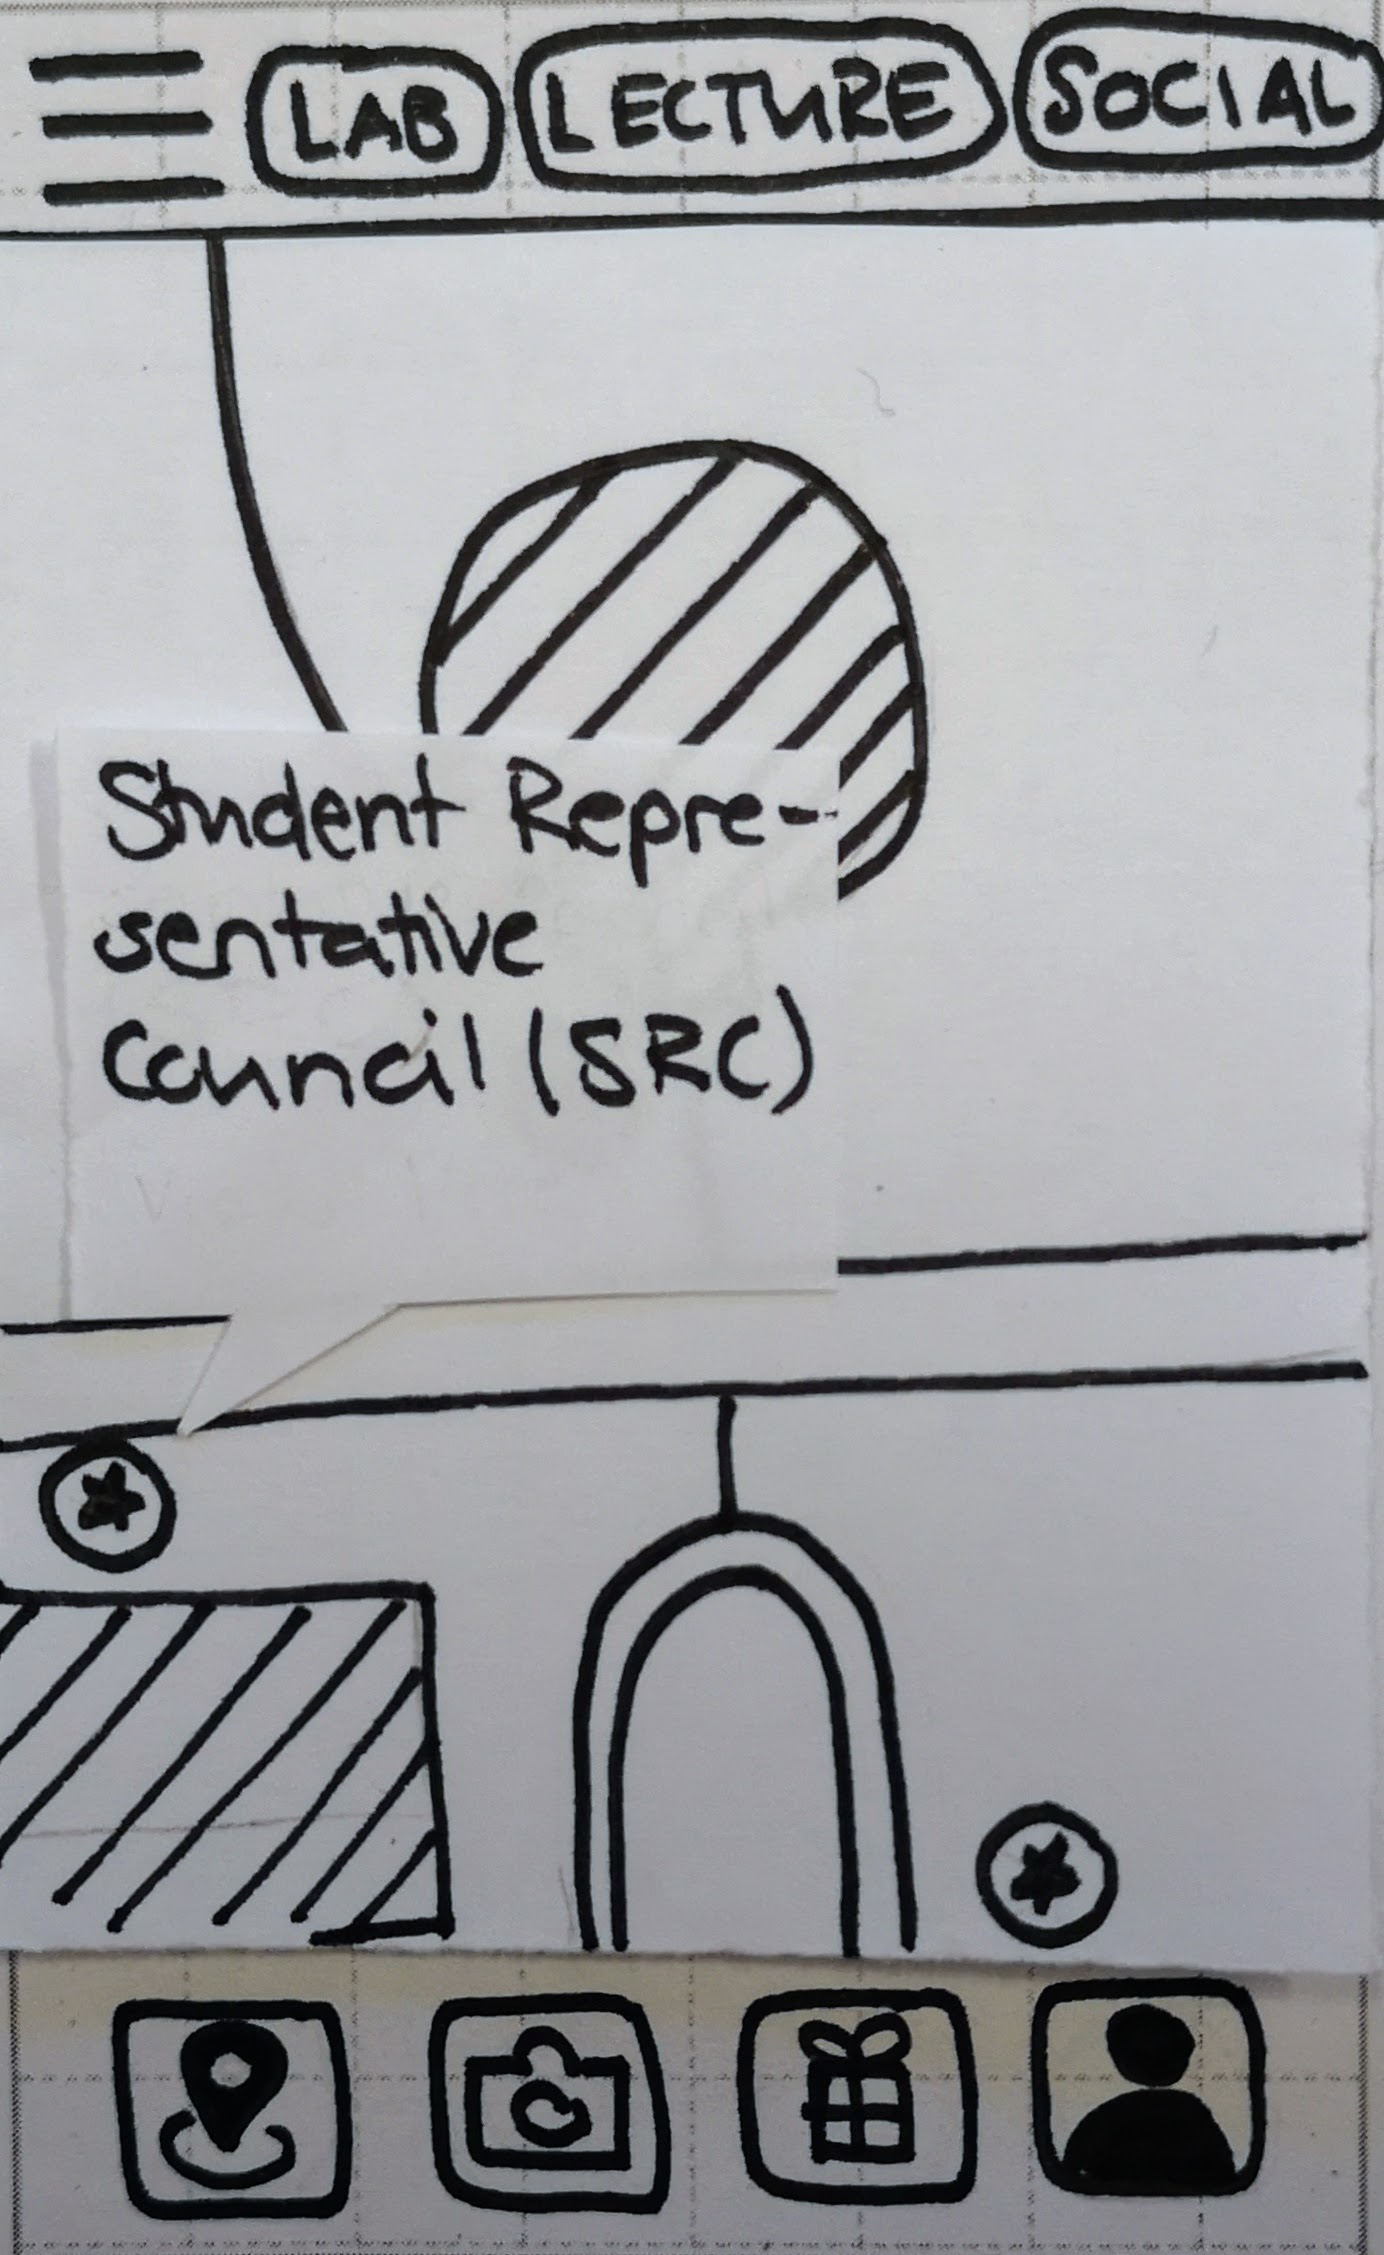
\includegraphics[width=0.4\textwidth]{./figures/map_src.jpg}
\caption{The screen if a point of interest (star is clicked). A pup-up will display the name of the place and some interesting facts.}
\label{fig:map_src}
\end{figure}

Points of interest are highlighted on the map. They can be clicked, which will then display more information about the places.

On the top of the screen, the different riddle icons are shown next to the classic menu icon (burger menu). If one of them is pushed, a related riddle pops up as shown in figure \ref{fig:map_riddle}. The riddles are displayed as a scroll that can be rolled up (swiped) or down to hide or display hints. Hints are displayed in text format; no arrows or direct navigation is shown.

\begin{figure}[ht]
\centering
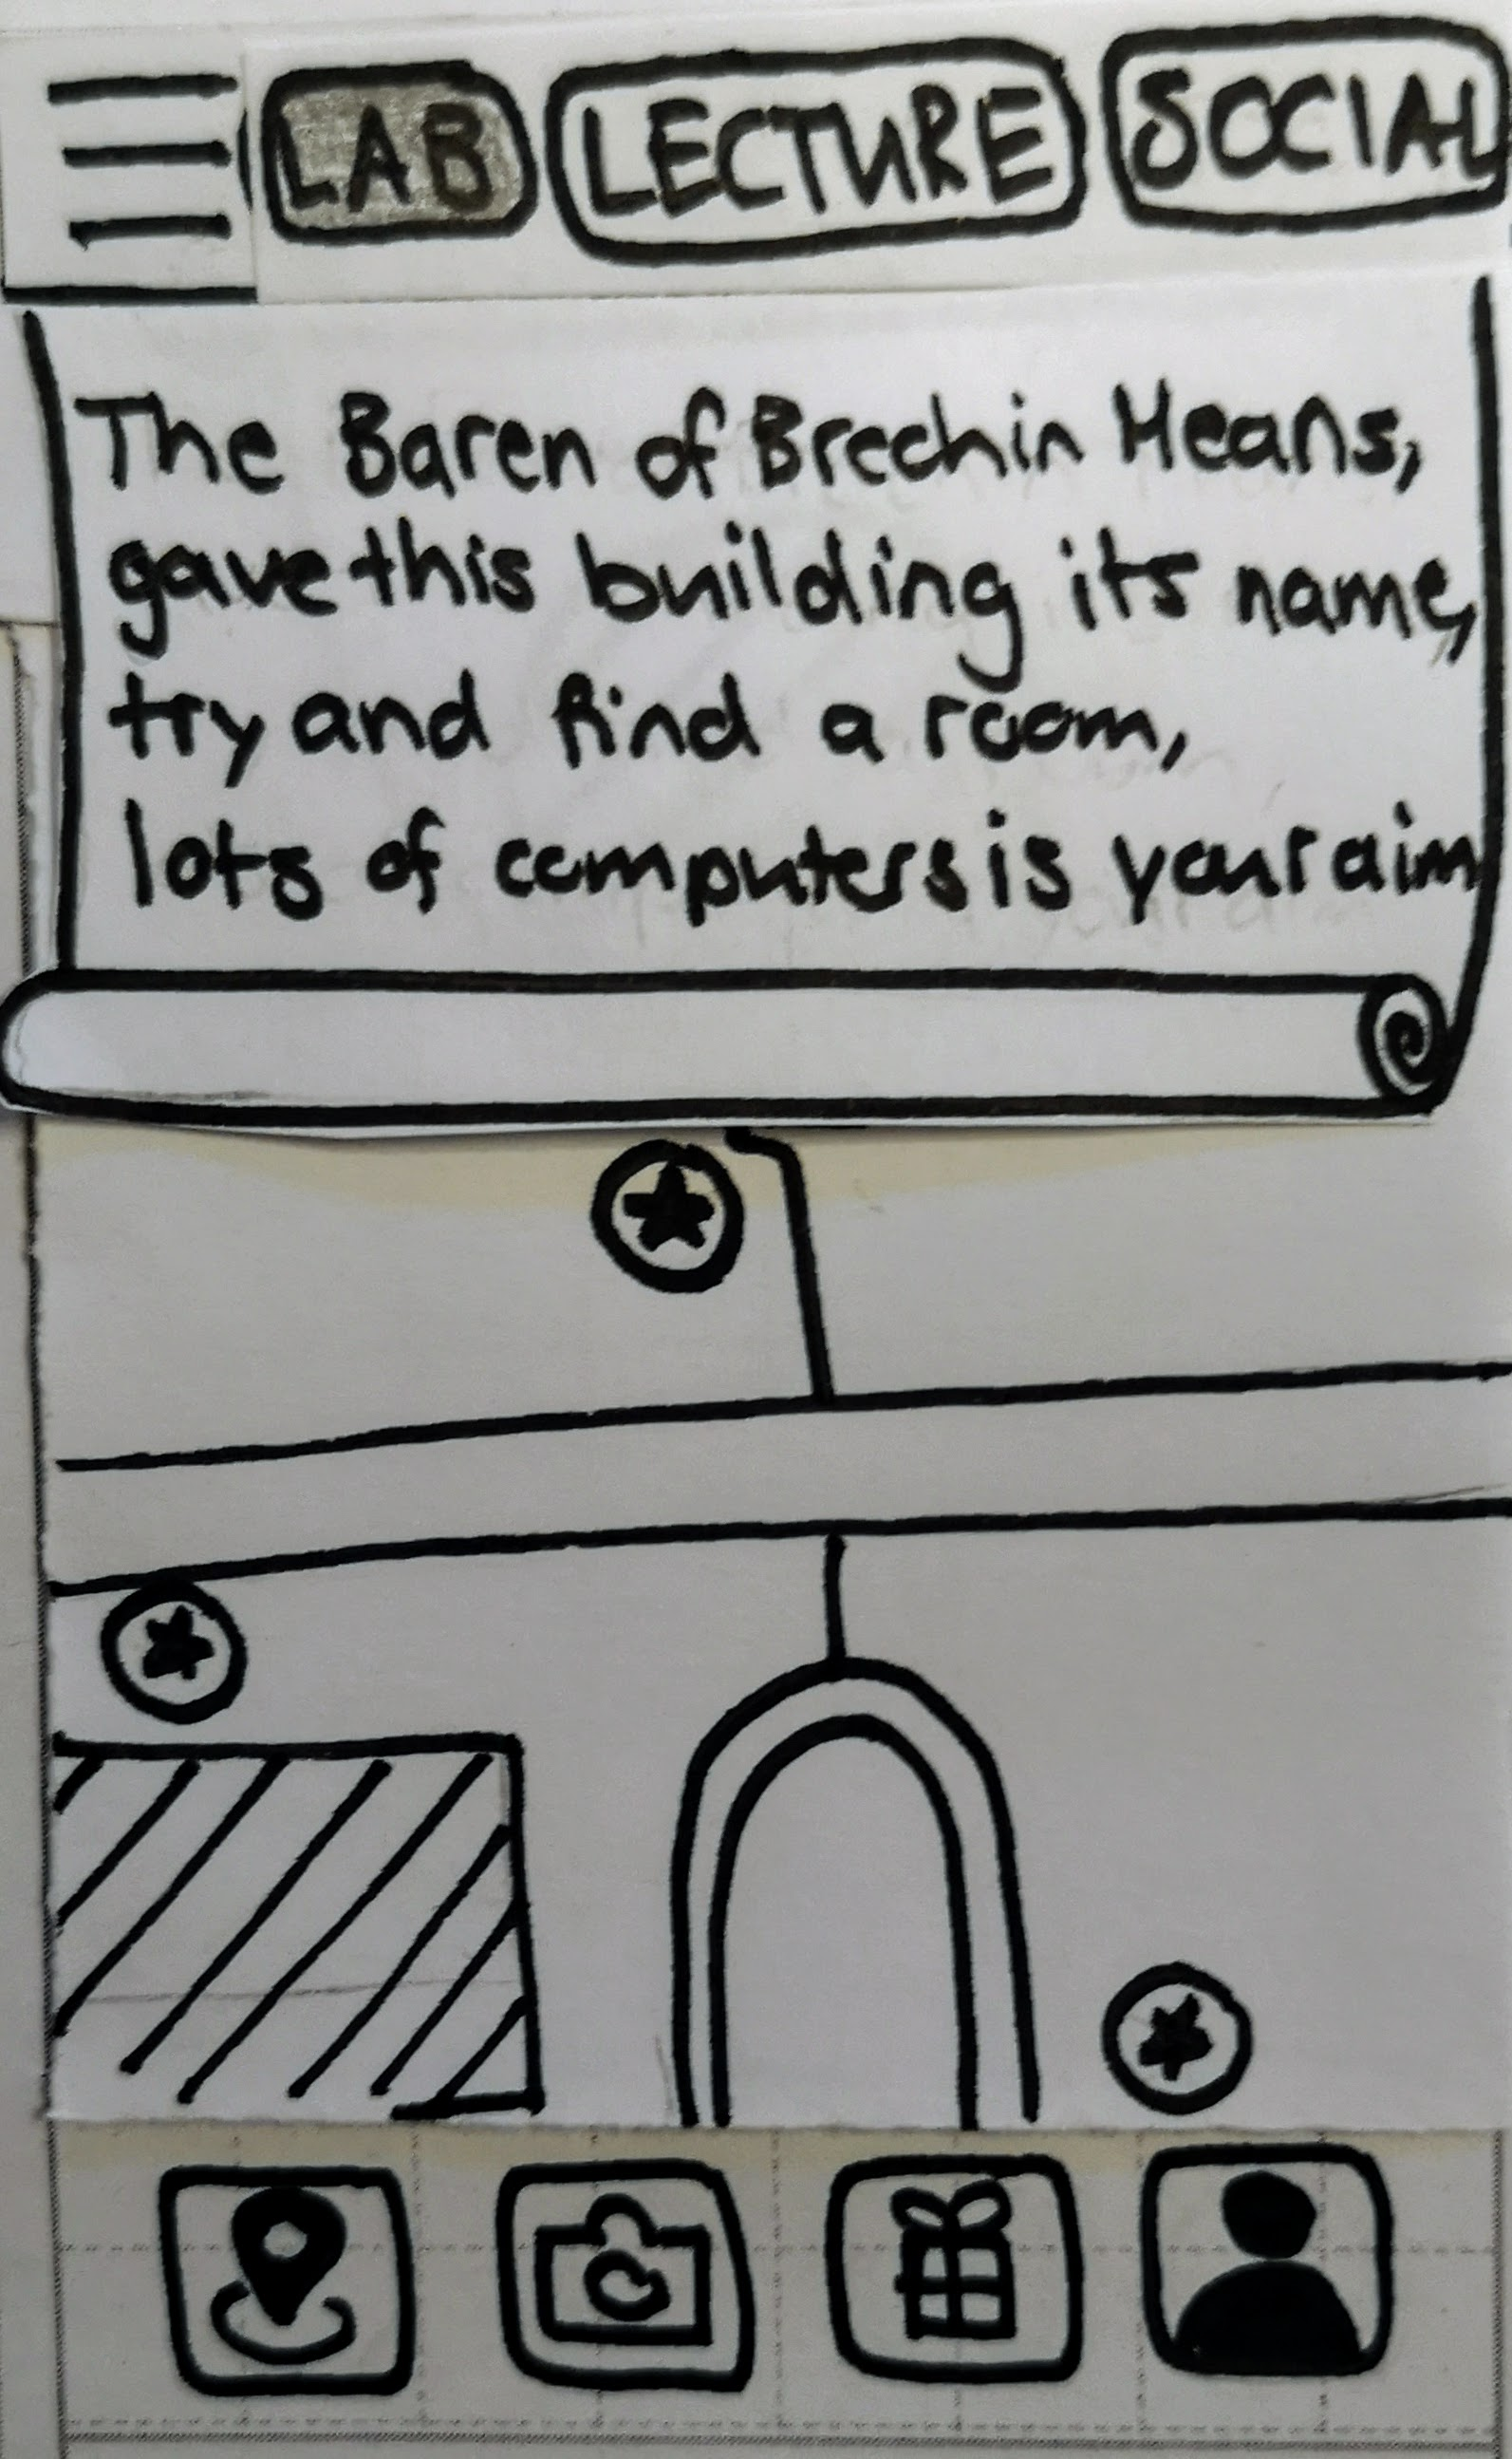
\includegraphics[width=0.4\textwidth]{./figures/map_riddle.jpg}
\caption{If a riddle is clicked, it is shown as text on a scroll. This scroll can be rolled back up to hide the riddle or scrolled further down, to show a hint.}
\label{fig:map_riddle}
\end{figure}

There should be an option to add friends with a QR-code (can be scanned with the camera) or by entering a user name the friends tab is no longer accessible directly from the main screen, but stored away in the profile section. 

\subsection*{Implementation and Evaluation Clickable Prototype}
This prototype was drawn up again and made interactive with the Marvel App. It which has very similar features as Invision, which was introduced in the lectures. The advantage of Marvel is that it allows an unlimited number of prototypes in the free version. Both programs allow the designer to implement interactions on drawings or on pictures that can be made directly in the program. The later was used.


\subsection*{User Testing}

This clickable prototype was sent to the testers through a link. They were  able to click through the displayed web page like an app. Every tester was initially briefed about the general concept of the app and subsequently filmed while they were interacting with it. They were asked to comment on what they are seeing and doing. The designer, who was filming this process, gave them pointers on what to do or helped them if they got stuck, especially if that was due to limitations of the clickable prototype. 

The tests were done with eight people. Various students from different backgrounds participated in the evaluations. Admittedly, most were from an engineering or computer science background, but there was also a philosophy and a biology student. The age of the testers ranges from 20 to 30 years. 

\paragraph{Limitations of the Prototype}
The mobile phone on which the prototype is vital for testing. A few phones had a different aspect ratio than the one anticipated by the Marvel App (the project is set up with a template for HTC One) can cause problems. If the screen is too wide and not long enough, the application introduces vertical scrolling. This makes using the up and down scrolling interaction difficult, because it interferes with the scrolling of the Marvel App.

Additionally, not every button was correctly linked to every screen at all times. This could be explained easily to the testers, by saying they took the right action, it is just not implemented.

Some testers had problems with the limited functions of the prototype. They had problems understanding that this is not actually a real application.

\paragraph{Results}
The transcripts from the user tests are not included here. Instead, generalised results are discussed. 

Most testers liked the simplistic design of the prototype, which was mainly due to the limitations of the prototype itself. However, this simplicity should be included in the next stage. Even though the icons are very rough, testers had no problem identifying their purpose. 

The testers often tried to just click on the map in the background to get back to the main screen when the riddle or a point of interest was displayed. 

The swiping actions were not automatically identified. Both in the offers section and when hiding a riddle or displaying a hint for it.

The testers all liked the gamification aspect of the app. They also enjoyed the points of interest and asked for more information like where the toilets or water fountains are. 

Every single tester that found the badges tried to click on them, to find out what they are about. No one expected to be much functionality, but they all wanted to enlarge the icon. 

The AR scanning function could not be tested properly. However, the app worked very well without it. Moreover, the question mark that is shown when "scanning" an AR tag seemed to confuse the testers and they did not always understand that they have to tap it. In theory, that step could be skipped without loosing any core functionality of the app idea.

\todo{belinda, write some more}
\subsection*{Implications for Next Stage}
The following recommendations were identified during the user test:
\begin{itemize}[noitemsep]
  \item If no riddle is selected, a message should be shown below the buttons: "click to get your first riddle".
  \item The information pop-up about point of interest should still allow all other interactions and not have to be clicked away first.  
  \item More information about a point of interest should be displayed. (Trivia, where are the toilets or water fountains?)
  \item Show the user in a better way that he can swipe to get to other offers. The arrows indicate clicking, but users usually want to swipe. 
  \item Remove the menu button. It is not needed an a settings menu can easily be stored away in the profile. This also increases the available space for the top buttons.  
  \item Hints need to be added when in scan mode ("ready to scan tag" / "click to activate").
  \item Hints need to be added to the riddles ("scroll down to get a hint", "scroll up to hide"), or at least arrows that point in the direction. Possibly allow click to reveal a new hint. If the user clicks anywhere on the map, that should hide the riddle.
  \item A prompt, like "are you sure you want to use a hint", should avoid accidentally using a hint for a riddle.
  \item Badges seem to be a good way to keep things interesting, people want to uncover the missing badges, the discovered ones should have some explanation, when clicked on ("discovered 5 cafés").
- add explations to badges (show them as pop-ups when clicking on them, display name, e.g. )
  \item An indication is needed for which navigation button at the bottom is active.(Selected register card.)
  \item Scanning a "wrong" solution should have more information. For example: "you get more points if you find this place with a riddle".
\end{itemize}
Additionally, some potential improvements have been identified that need to be explored further:
\begin{itemize}[noitemsep]
  \item Add the ability to see friends profile in more detail.
  \item Add more interaction with friends, like joint riddles or the ability to send gifts to friends.
  \item Show the riddle if the place is claimed without a riddle "just for the fun of it".
  \item Show the solved riddles in the map screen when clicking on the stars.
  \item Is AR really necessary? It certainly is a nice gimmick, but not specifically needed, scanning a code seems to be enough for the functionality.
\end{itemize}
% ------------------------------------
\section*{Demonstrator Prototype}

Lorem ipsum dolor sit amet, consectetur adipiscing elit, sed do eiusmod tempor incididunt ut labore et dolore magna aliqua. Ut enim ad minim veniam, quis nostrud exercitation ullamco laboris nisi ut aliquip ex ea commodo consequat. Duis aute irure dolor in reprehenderit in voluptate velit esse cillum dolore eu fugiat nulla pariatur. Excepteur sint occaecat cupidatat non proident, sunt in culpa qui officia deserunt mollit anim id est laborum.

\section*{Appendices}
\subsection*{Appendix A}
\subsubsection*{Prototype 1}


\end{document}
